%%%%%%%%%%%%%%%%%%%%%%%%%%%%%%%%%%%%%%%%%
% Short Sectioned Assignment LaTeX Template Version 1.0 (5/5/12)
% This template has been downloaded from: http://www.LaTeXTemplates.com
% Original author:  Frits Wenneker (http://www.howtotex.com)
% License: CC BY-NC-SA 3.0 (http://creativecommons.org/licenses/by-nc-sa/3.0/)
%%%%%%%%%%%%%%%%%%%%%%%%%%%%%%%%%%%%%%%%%

%----------------------------------------------------------------------------------------
%   PACKAGES AND OTHER DOCUMENT CONFIGURATIONS
%----------------------------------------------------------------------------------------

\documentclass[10pt,a4paper,spanish]{article}

% ---- Entrada y salida de texto -----

\usepackage[spanish]{babel} 
\usepackage[T1]{fontenc} % Use 8-bit encoding that has 256 glyphs
\usepackage[utf8]{inputenc}
\usepackage{cite}
% \usepackage{spreadtab}
% \usepackage{fourier} % Use the Adobe Utopia font for the document - comment this line to return to the LaTeX default
\usepackage[usenames, dvipsnames]{color}
\usepackage[table]{xcolor}
\usepackage{colortbl}
\usepackage[bookmarks=true,colorlinks=true,linkcolor=red,citecolor=blue]{hyperref}
% \usepackage{cite}
% \usepackage[official]{eurosym}
\usepackage{tikz}
% \usepackage{pgfplots}
% \pgfplotsset{compat=1.5}

\usepackage{subfigure}

% \usepackage{pseudocode}

% ---- Otros paquetes ----
\usepackage{enumerate}
\usepackage{amsmath,amsfonts,amsthm,amssymb} % Math packages
\usepackage{graphics,graphicx} %para incluir imágenes y notas en las imágenes
% Para hacer tablas comlejas
%\usepackage{multirow}
%\usepackage{threeparttable}

\usepackage[a4paper, margin=1.3in]{geometry}


\usepackage{sectsty} % Allows customizing section commands
\allsectionsfont{\centering \normalfont\bfseries\scshape} % Make all sections centered, the default font and small caps
\usepackage{fancyhdr}
\pagestyle{fancy}
%con esto nos aseguramos de que las cabeceras de capítulo y de sección vayan en minúsculas

\renewcommand{\sectionmark}[1]{%
      \markright{\thesection\ #1}}
\fancyhf{} %borra cabecera y pie actuales
\fancyhead[LE,RO]{{\bfseries Práctica 3}}
\fancyhead[LO]{\bfseries Marta Gómez}
\fancyfoot[C]{\thepage{}}
\renewcommand{\headrulewidth}{0.5pt}
\renewcommand{\footrulewidth}{0pt}
\addtolength{\headheight}{0.5pt} %espacio para la raya
\fancypagestyle{plain}{%
      \fancyhead{} %elimina cabeceras en páginas "plain"
      \renewcommand{\headrulewidth}{0pt} %así como la raya
}

\numberwithin{equation}{section} % Number equations within sections (i.e. 1.1, 1.2, 2.1, 2.2 instead of 1, 2, 3, 4)
\numberwithin{figure}{section} % Number figures within sections (i.e. 1.1, 1.2, 2.1, 2.2 instead of 1, 2, 3, 4)
\numberwithin{table}{section} % Number tables within sections (i.e. 1.1, 1.2, 2.1, 2.2 instead of 1, 2, 3, 4)

\setlength\parindent{0pt} % Removes all indentation from paragraphs - comment this line for an assignment with lots of text
\setlength{\parskip}{1ex plus 0.5ex minus 0.2ex}

\newcommand{\horrule}[1]{\rule{\linewidth}{#1}} % Create horizontal rule command with 1 argument of height

%----------------------------------------------------------------------------------------
%   TÍTULO Y DATOS DEL ALUMNO
%----------------------------------------------------------------------------------------

\title{
\normalfont \normalsize 
{\bf Redes y Sistemas Complejos} \\ Curso 2016-2017 \\ [25pt] % Your university, school and/or department name(s)
\horrule{0.5pt} \\[0.4cm] % Thin top horizontal rule
\huge \textsc{Práctica 3: \\ Estudio Comparativo de Métodos \\ para Poda y Visualización \\ de Redes } \\ % The assignment title
\horrule{2pt} \\[0.5cm] % Thick bottom horizontal rule
}

\author{\textit{Marta Gómez Macías}} %\\ \texttt{mgmacias95@correo.ugr.es} \\ 75929776Z \\[0.5cm]

% \date{\normalsize\today} % Incluye la fecha actual

% \usepackage{pdflscape}

%----------------------------------------------------------------------------------------
% DOCUMENTO
%----------------------------------------------------------------------------------------

\begin{document}
%Cambiar Cuadros por Tablas y lista de...
\renewcommand{\listtablename}{Índice de tablas}
\renewcommand{\tablename}{Tabla} 

\begin{titlepage}
\begin{center}

\includegraphics[width=0.2\textwidth]{../../ugr}

\normalfont \normalsize 
{\bf Redes y Sistemas Complejos} \\ Curso 2016-2017 \\ [25pt] % Your university, school and/or department name(s)
\horrule{0.5pt} \\[0.4cm] % Thin top horizontal rule
{\huge \textsc{Práctica 3: \\ Estudio Comparativo de Métodos \\ para Poda y Visualización \\ de Redes }} % The assignment title
\horrule{2pt} \\[0.5cm] % Thick bottom horizontal rule

{\Large \textit{Marta Gómez Macías} \\ \texttt{mgmacias95@correo.ugr.es} \\ 75929776Z \\[0.5cm]

\date{\today}} % Incluye la fecha actual
\end{center}
\end{titlepage}

\tableofcontents % para generar el índice de contenidos

% \listoffigures

% \listoftables

\section{Poda y visualización de redes con tamaño pequeño.}


\subsection{Variante de \textit{Pathfinder} y cienciogramas escogidos}
La variante de \textit{Pathfinder} escogida para realizar esta parte de la práctica ha sido \textbf{Binary Pathfinder} debido a su mayor eficiencia y menor uso de memoria. Respecto a los cienciogramas escogidos, he lanzado un generador de números aleatorios y he obtenido los siguientes:

\begin{enumerate}[\qquad\ ---]
    \item Chile (2004)
    \item Mexico (2005)
    \item Spain (2002)
    \item USA (2002)
    \item Japan (2002)
    \item Argentina (2005)
    \item Germany (2002)
    \item Canada (2005)
    \item Cuba (2004)
    \item World (2002)
\end{enumerate}

% Para usar el programa: ./binary-pathfinder ../cienciogramas/<filename> <q>

\subsection{Resultados obtenidos en cada cienciograma}

\begin{table}[!h]
\begin{minipage}{0.5\textwidth}
\centering
\begin{tabular}{lrr}
\hline
 Argentina-2005 & \multicolumn{2}{c}{$r = \infty$} \\
($n=266$)   &   Nº  enlaces &    Densidad \\
\hline
 Red original                 &               $17938$ & $0.508952$ \\
 $2$                            &                 $324$ & $0.00619195$  \\
 $3$                            &                 $277$ & $0.00919279$  \\
 $4$                            &                 $269$ & $0.00763229$  \\
 $5$                            &                 $268$ & $0.00760392$  \\
 $265$                          &                 $267$ & $0.00757554$   \\
\hline
\end{tabular}
\caption{Resultados obtenidos en el cienciograma Argentina-2005}
\label{argentina2005}
\end{minipage}
\begin{minipage}{0.5\textwidth}
\centering
\begin{tabular}{lrr}
\hline
 Canada-2005 & \multicolumn{2}{c}{$r = \infty$} \\
($n=288$)   &   Nº  enlaces &    Densidad \\
\hline
 Red original              &               $30574$ & $0.739789$ \\
 $2$                         &                 $340$ & $0.00822687$  \\
 $3$                         &                 $301$ & $0.0072832$  \\
 $4$                         &                 $290$ & $0.00701703$  \\
 $5$                         &                 $287$ & $0.00694444$  \\
 $287$                       &                 $287$ & $0.00694444$  \\
\hline
\end{tabular}
\caption{Resultados obtenidos en el cienciograma Canada-2005}
\label{canada2005}
\end{minipage}
\end{table}

\begin{table}[!h]
\begin{minipage}{0.5\textwidth}
\centering
\begin{tabular}{lrr}
\hline
 Chile-2004 & \multicolumn{2}{c}{$r = \infty$} \\
($n=256$)   &   Nº  enlaces &    Densidad \\
\hline
 Red original             &               $14778$ & $0.452757$ \\
 $2$                        &                 $318$ & $0.00974265$  \\
 $3$                        &                 $265$ & $0.00811887$  \\
 $4$                        &                 $258$ & $0.00790441$   \\
 $5$                        &                 $256$ & $0.00784314$  \\
 $255$                      &                 $256$ & $0.00784314$  \\
\hline
\end{tabular}
\caption{Resultados obtenidos en el cienciograma Chile-2004}
\label{chile2004}
\end{minipage}
\begin{minipage}{0.5\textwidth}
\centering
\begin{tabular}{lrr}
\hline
 Cuba-2004 & \multicolumn{2}{c}{$r = \infty$} \\
($n=237$)   &   Nº  enlaces &   Densidad \\
\hline
 Red original            &                $9518$ & $0.340342$ \\
 $2$                       &                 $285$ & $0.0101909$ \\
 $3$                       &                 $255$ & $0.00911821$ \\
 $4$                       &                 $249$ & $0.00890367$ \\
 $5$                       &                 $247$ & $0.00883215$ \\
 $236$                     &                 $247$ & $0.00883215$ \\
\hline
\end{tabular}
\caption{Resultados obtenidos en el cienciograma Cuba-2004}
\label{cuba2004}
\end{minipage}
\end{table}

\begin{table}[!h]
\begin{minipage}{0.5\textwidth}
\centering
\begin{tabular}{lrr}
\hline
 Spain-2002 & \multicolumn{2}{c}{$r = \infty$} \\
($n=264$)   &   Nº enlaces &    Densidad \\
\hline
 Red original             &               $21807$ & $0.628154$ \\
 $2$                        &                 $320$ & $0.00921765$  \\
 $3$                        &                 $274$ & $0.00789261$  \\
 $4$                        &                 $265$ & $0.00763337$  \\
 $5$                        &                 $263$ & $0.00757576$  \\
 $263$                      &                 $263$ & $0.00757576$  \\
\hline
\end{tabular}
\caption{Resultados obtenidos en el cienciograma Spain-2002}
\label{spain2002}
\end{minipage}
\begin{minipage}{0.5\textwidth}
\centering
\begin{tabular}{lrr}
\hline
 Germany-2002 & \multicolumn{2}{c}{$r = \infty$} \\
($n=269$)   &   Nº enlaces &    Densidad \\
\hline
 Red original               &               $25395$ & $0.704516$ \\
 $2$                          &                 $313$ & $0.00868335$  \\
 $3$                          &                 $277$ & $0.00768463$  \\
 $4$                          &                 $272$ & $0.00754591$  \\
 $5$                          &                 $270$ & $0.00749043$  \\
 $268$                        &                 $269$ & $0.00746269$  \\
\hline
\end{tabular}
\caption{Resultados obtenidos en el cienciograma Germany-2002}
\label{germany2002}
\end{minipage}
\end{table}

\begin{table}[!h]
\begin{minipage}{0.5\textwidth}
\centering
\begin{tabular}{lrr}
\hline
 Japan-2002 & \multicolumn{2}{c}{$r = \infty$} \\
($n=265$)   &   Nº enlaces &    Densidad \\
\hline
 Red original             &               $21754$ & $0.621898$ \\
 $2$                        &                 $316$ & $0.00903373$  \\
 $3$                        &                 $279$ & $0.00797599$  \\
 $4$                        &                 $269$ & $0.00769011$  \\
 $5$                        &                 $267$ & $0.00763293$   \\
 $264$                      &                 $267$ & $0.00763293$   \\
\hline
\end{tabular}
\caption{Resultados obtenidos en el cienciograma Japan-2002}
\label{japan2002}
\end{minipage}
\begin{minipage}{0.5\textwidth}
\centering
\begin{tabular}{lrr}
\hline
 Mexico-2005 & \multicolumn{2}{c}{$r = \infty$} \\
($n=270$)   &   Nº enlaces &   Densidad \\
\hline
 Red original              &               $20110$ & $0.553766$ \\
 $2$                         &                 $336$ & $0.00925238$ \\
 $3$                         &                 $284$ & $0.00782046$ \\
 $4$                         &                 $275$ & $0.00757263$ \\
 $5$                         &                 $274$ & $0.00754509$ \\
 $269$                       &                 $273$ & $0.00751755$ \\
\hline
\end{tabular}
\caption{Resultados obtenidos en el cienciograma Mexico-2005}
\label{mexico2005}
\end{minipage}
\end{table}

\begin{table}[!h]
\begin{minipage}{0.5\textwidth}
\centering
\begin{tabular}{lrr}
\hline
 US-2002 & \multicolumn{2}{c}{$r = \infty$} \\
($n=276$)   &   Nº enlaces &    Densidad \\
\hline
 Red original                     &               $31292$ & $0.824559$ \\
 $2$                                &                 $314$ & $0.00827404$  \\
 $3$                                &                 $287$ & $0.00756258$  \\
 $4$                                &                 $279$ & $0.00735178$  \\
 $5$                                &                 $277$ & $0.00729908$  \\
 $275$                              &                 $275$ & $0.00724638$  \\
\hline
\end{tabular}
\caption{Resultados obtenidos en el cienciograma United\_States-2002}
\label{unitedstates2002}
\end{minipage}
\begin{minipage}{0.5\textwidth}
\centering
\begin{tabular}{lrr}
\hline
 World & \multicolumn{2}{c}{$r = \infty$} \\
($n=218$)   &   Nº enlaces &    Densidad \\
\hline
 Red original        &               $20154$ & $0.85207$ \\
 $2$                   &                 $280$ & $0.0118378$  \\
 $3$                   &                 $233$ & $0.00985076$  \\
 $4$                   &                 $223$ & $0.00942798$  \\
 $5$                   &                 $220$ & $0.00930115$  \\
 $217$                 &                 $217$ & $0.00917431$  \\
\hline
\end{tabular}
\caption{Resultados obtenidos en el cienciograma World}
\label{world}
\end{minipage}
\end{table}

\subsection{Análisis de los resultados obtenidos en cada cienciograma}
La tónica general en todos los cienciogramas es una reducción drástica del número de enlaces entre la red original ($q = 1$) y una poda con $q = 2$. Esta primera poda es bastante fuerte, ya que elimina la gran mayoría de nodos, por ejemplo, en el cienciograma de los Estados Unidos en el año 2002 (\hyperref[unitedstates2002]{Tabla \ref*{unitedstates2002}}) pasamos de 31292 enlaces a 314, es decir, tras la poda sólo quedan el $1.0034\%$ de los nodos. Algo parecido pasa en el cienciograma de Canadá en el año 2005, donde pasamos de 30574 enlaces a 340, dejando sólo un $1.11\%$ de los enlaces. Una vez hecha la primera poda, las sucesivas son bastante más suaves, por tanto, podemos concluir que \textbf{la intensidad de la poda es inversamente proporcional al valor de $q$}: cuanto más pequeño sea $q$, mayor será la poda. Obviamente, $q \geq 2$ ya que $q = 1$ corresponde a la red original.

Como hemos dicho antes, la intensidad de la poda se reduce conforme se aumenta el valor de $q$, ahora bien, llega un momento en el que ya no se puede podar más. En la mayoría de cienciogramas estudiados, este momento llega cuando $q = 5$, ahora bien, no siempre es así, ya que hay ejemplos en los que desde $q = 5$ hasta $q = n-1$ podan varios enlaces más: World (\hyperref[world]{Tabla \ref*{world}}), United States 2002 (\hyperref[unitedstates2002]{Tabla \ref*{unitedstates2002}}), Argentina 2005 (\hyperref[argentina2005]{Tabla \ref*{argentina2005}}), entre otros. Por tanto, podemos concluir que \textbf{A partir de, más o menos, $q = 5$ la PFNET($r = \infty$, $q$) alcanza su valor máximo de poda}, además, \textbf{no hay mucha dispersión en ese valor}, ya que casi todos los cienciogramas llegan al límite ahí.

Otro detalle a tener en cuenta es que conforme se va podando la red, va reduciéndose la densidad de la misma. Para entender por qué ocurre esto, es necesario saber la fórmula de la densidad:

\begin{displaymath}
    D = \frac{L}{L_{max}} \qquad\ \textrm{Donde } L_{max} = \frac{N(N-1)}{2}
\end{displaymath}

es decir, la densidad depende del número de enlaces, $L$, de la red, al ir eliminando enlaces al podar, también reducimos la densidad de la red.

\subsection{Visualización de los cienciogramas y comparación de los métodos de distribución K-K y F-R}

Los cienciogramas que he elegido para visualizar son la de \textit{Estados Unidos en el año 2002} (Figuras \hyperref[frus]{\ref*{frus}} y \hyperref[kkus]{\ref*{kkus}} y \hyperref[unitedstates2002]{Tabla \ref*{unitedstates2002}}) porque es la que más poda entre $q = 5$ y $q = n-1$ y la de \textit{España en el año 2002} (Figuras \hyperref[frsp]{\ref*{frsp}} y \hyperref[kksp]{\ref*{kksp}} y \hyperref[spain2002]{Tabla \ref*{spain2002}}) porque no poda nada una vez pasado $q = 5$.

Para poder aplicar el método K-K, he tenido que anular la fuerza de atracción, ya que si no, los nodos salían demasiado pegados en las visualizaciones. A pesar de esto, he obtenido una distribución en forma de estrella en vez de la típica distribución de mapa de metro.

Con ambas redes, debido a que tienen una naturaleza muy similar, obtenemos resultados muy parecidos. Incluso, las visualizaciones las redes con cada método de distribución y distinto $q$ han dado resultados prácticamente idénticos. Por tanto, el análisis se centrará más en diferenciar al método K-K y al F-R.

Con el método F-R, obtenemos una visualización prácticamente \textit{circular}, y en el centro se ven los enlaces con un mayor peso. En cambio, con el método K-K, obtenemos un grafo de estrella, donde en el centro se colocan una serie de nodos equidistantes entre sí y otros en las puntas de las estrellas. Otro detalle a destacar del K-K, es que ha dejado los enlaces con más peso en los nodos de la periferia, al contrario que el método F-R. Por tanto, podemos concluir que hemos obtenido grafos completamente distintos con ambos métodos.

Estas diferencias se deben a las diferencias en la naturaleza de ambos algoritmos: el F-R tiende a colocar próximos los nodos que estén conectados entre sí mientras que el K-K, se persigue conseguir las distancias teóricas que existen en el grafo. En nuestro caso, hemos tenido que anular la fuerza atractiva del K-K para que los nodos no se solapasen entre sí en un único nodo por lo que sólo hemos dejado actuar a la fuerza repulsiva. Así, con el método de distribución F-R se han colocado los nodos con más enlaces en el centro del grafo y los que tenían menos, han ido a parar a la periferia del grafo. En cambio, en el K-K, hay nodos en la periferia con muchos más enlaces que los nodos del centro.

Ambas distruciones dan bastante información sobre la red, aunque necesitan de información adicional como tamaño de los nodos o un coloreado.

\begin{figure}[!h]
    \centering
    \mbox{
        \subfigure[PFNET($r = \infty$, $q = 2$)]{
            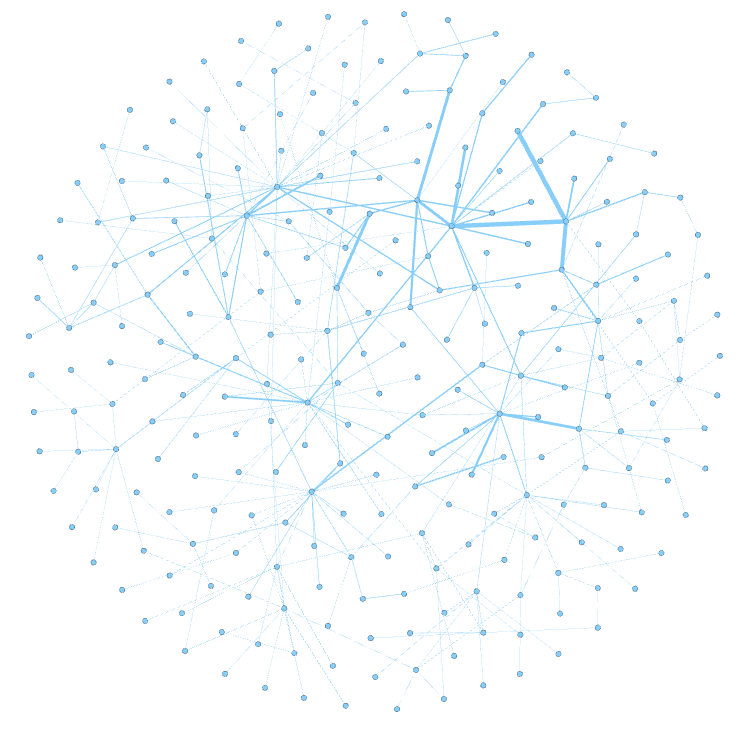
\includegraphics[width=0.25\textwidth]{../visualizacion/q2_fr_spain}
            \label{q2frsp}
        }
        \subfigure[PFNET($r = \infty$, $q = 3$)]{
            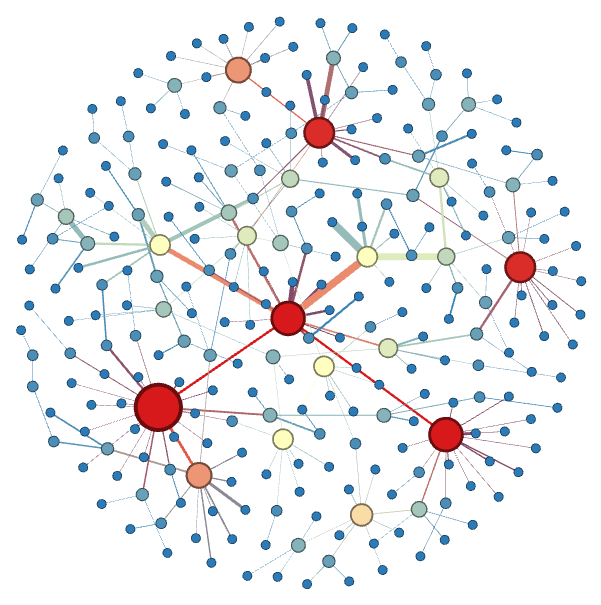
\includegraphics[width=0.25\textwidth]{../visualizacion/q3_fr_spain}
            \label{q3frsp}
        }
    }
    \mbox{
        \subfigure[PFNET($r = \infty$, $q = 4$)]{
            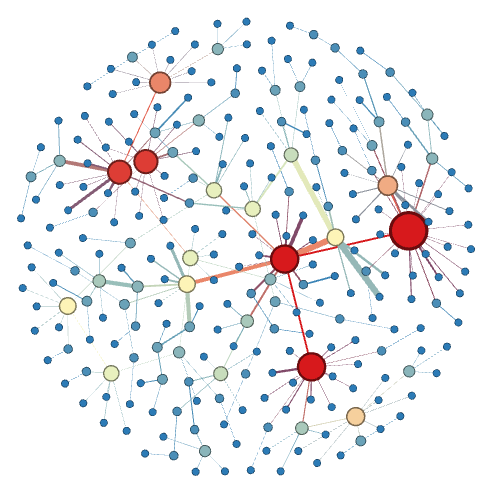
\includegraphics[width=0.25\textwidth]{../visualizacion/q4_fr_spain}
            \label{q4frsp}
        }
        \subfigure[PFNET($r = \infty$, $q = n-1$)]{
            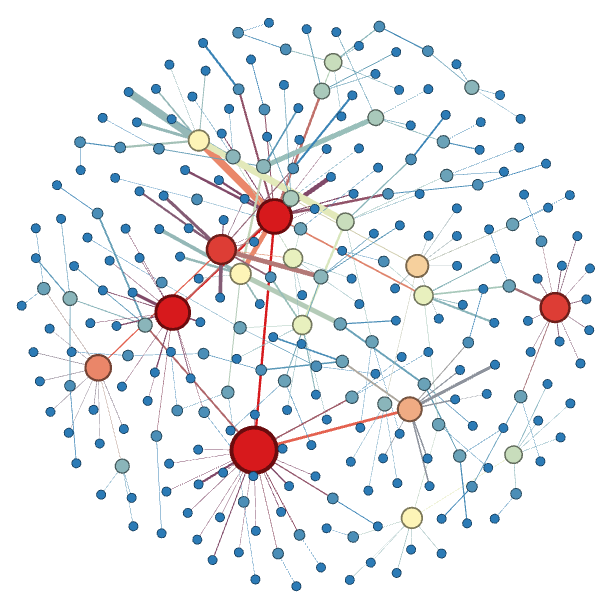
\includegraphics[width=0.25\textwidth]{../visualizacion/qn_fr_spain}
            \label{qnfrsp}
        }
    }
    \caption{Visualizaciones de las PFNETs del cienciograma Spain-2002 realizadas con el método de distribución F-R}
    \label{frsp}
\end{figure}

\begin{figure}[!h]
    \centering
    \mbox{
        \subfigure[PFNET($r = \infty$, $q = 2$)]{
            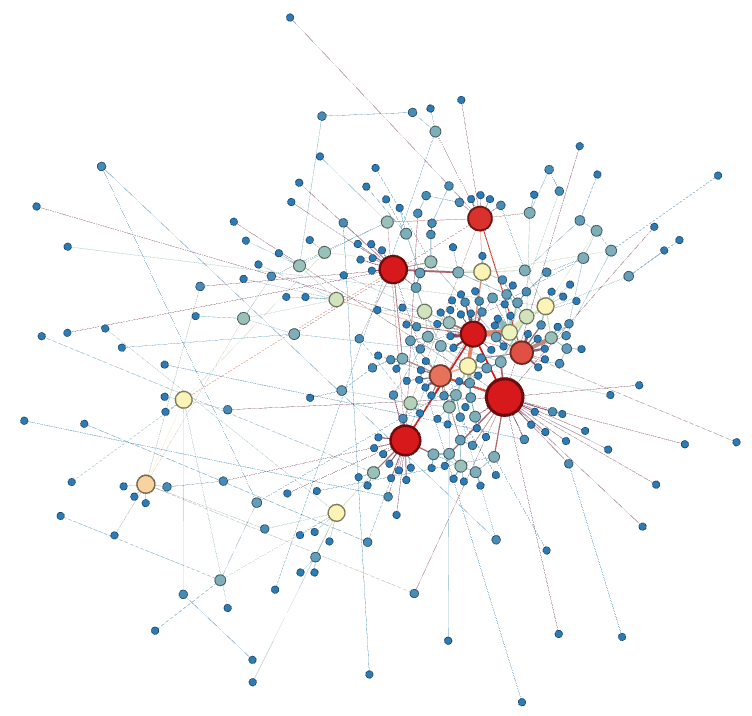
\includegraphics[width=0.25\textwidth]{../visualizacion/q2_kk_spain}
            \label{q2kksp}
        }
        \subfigure[PFNET($r = \infty$, $q = 3$)]{
            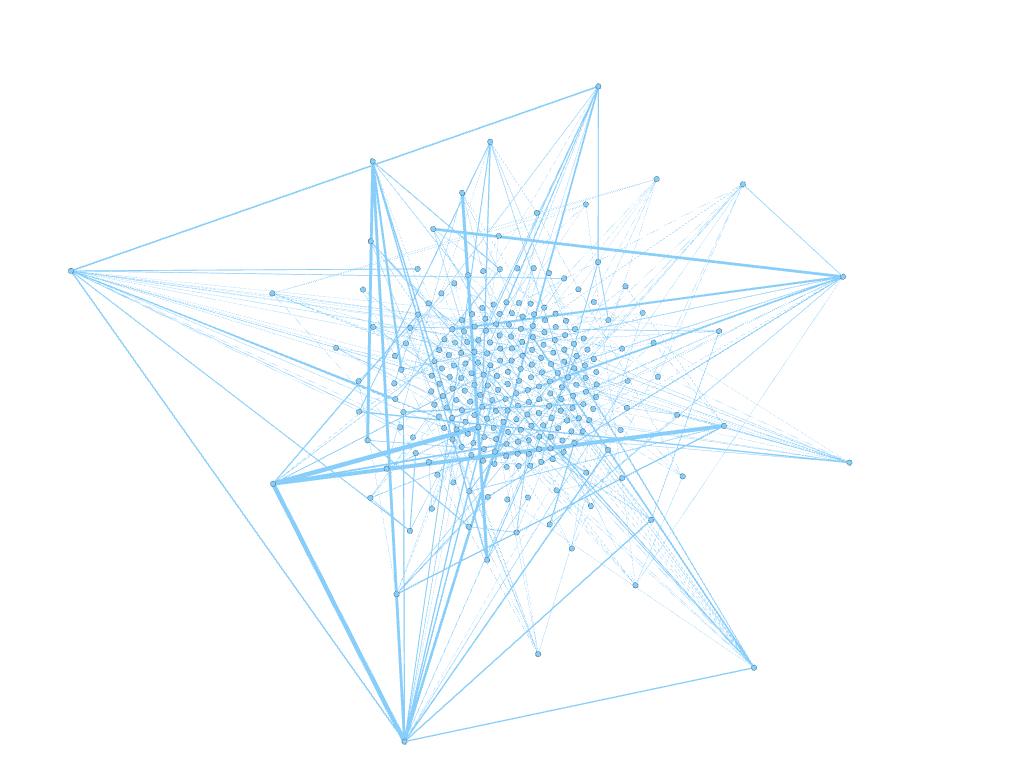
\includegraphics[width=0.25\textwidth]{../visualizacion/q3_kk_spain}
            \label{q3kksp}
        }
    }
    \mbox{
        \subfigure[PFNET($r = \infty$, $q = 4$)]{
            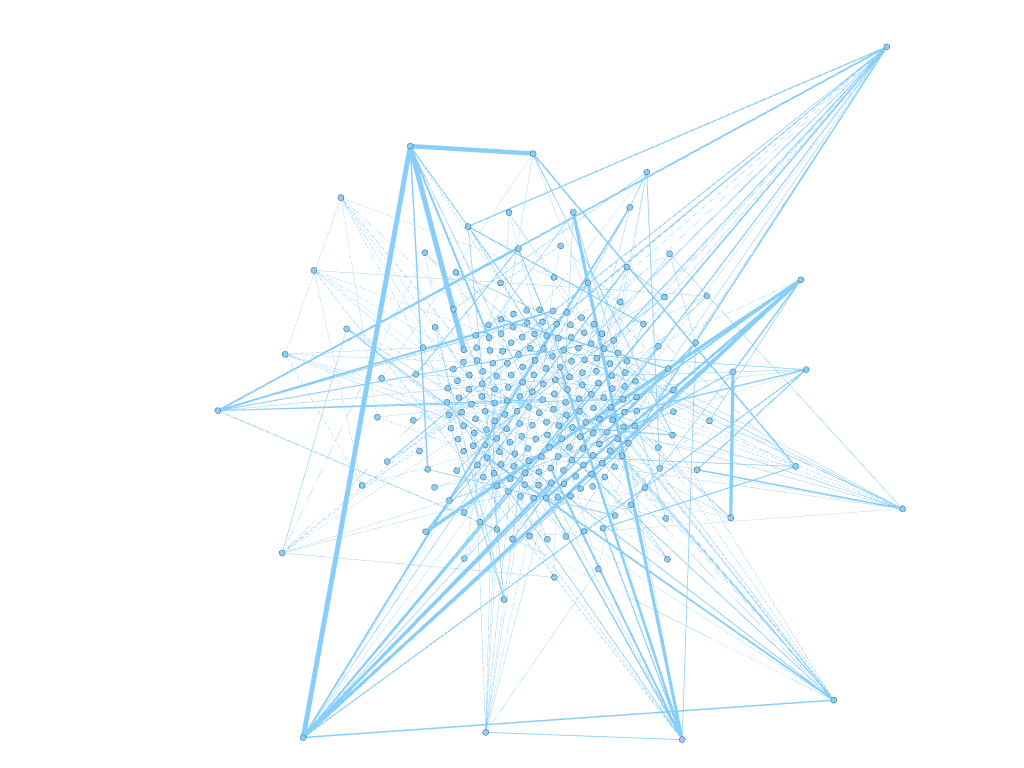
\includegraphics[width=0.25\textwidth]{../visualizacion/q4_kk_spain}
            \label{q4kksp}
        }
        \subfigure[PFNET($r = \infty$, $q = n-1$)]{
            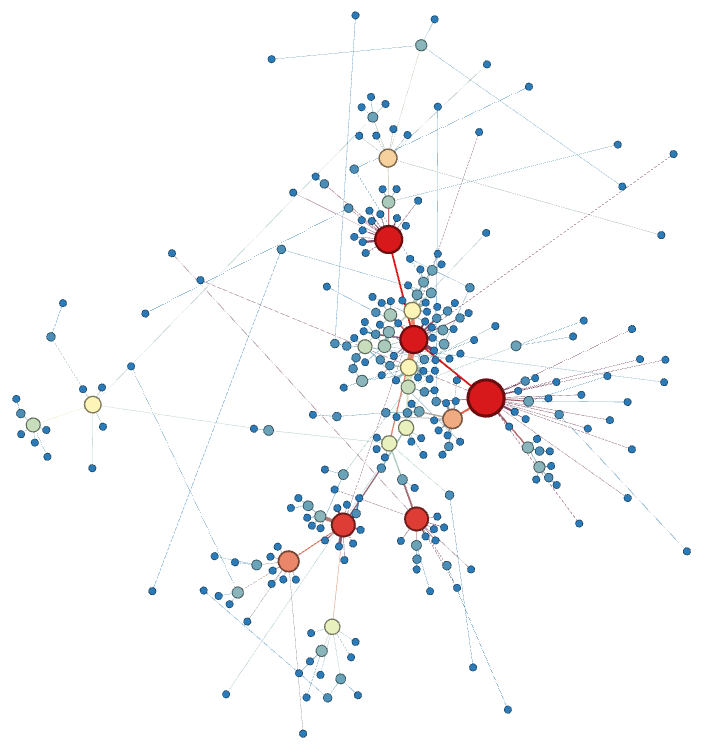
\includegraphics[width=0.25\textwidth]{../visualizacion/qn_kk_spain}
            \label{qnkksp}
        }
    }
    \caption{Visualizaciones de las PFNETs del cienciograma Spain-2002 realizadas con el método de distribución K-K}
    \label{kksp}
\end{figure}

\begin{figure}[!h]
    \centering
    \mbox{
        \subfigure[PFNET($r = \infty$, $q = 2$)]{
            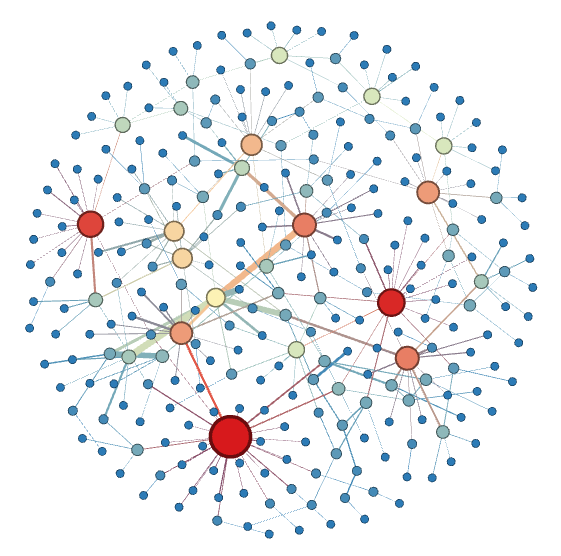
\includegraphics[width=0.25\textwidth]{../visualizacion/q2_fr_us}
            \label{q2frus}
        }
        \subfigure[PFNET($r = \infty$, $q = 3$)]{
            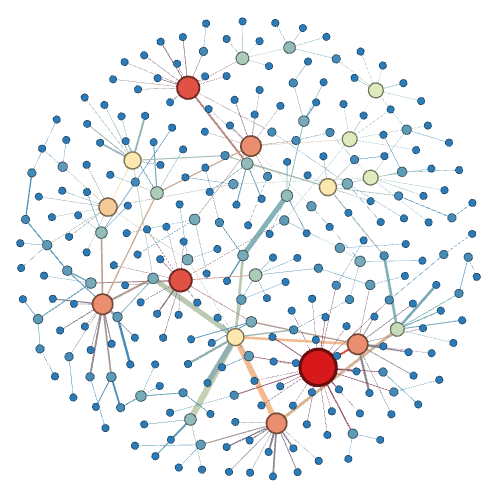
\includegraphics[width=0.25\textwidth]{../visualizacion/q3_fr_us}
            \label{q3frus}
        }
    }
    \mbox{
        \subfigure[PFNET($r = \infty$, $q = 4$)]{
            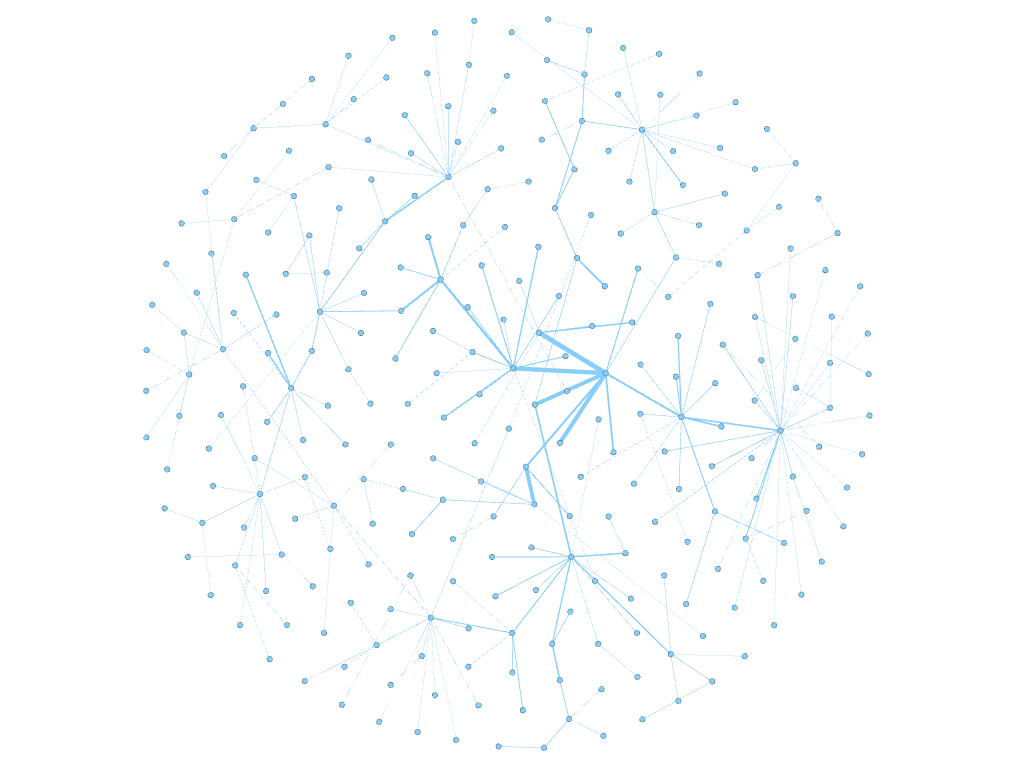
\includegraphics[width=0.25\textwidth]{../visualizacion/q4_fr_us}
            \label{q4frus}
        }
        \subfigure[PFNET($r = \infty$, $q = n-1$)]{
            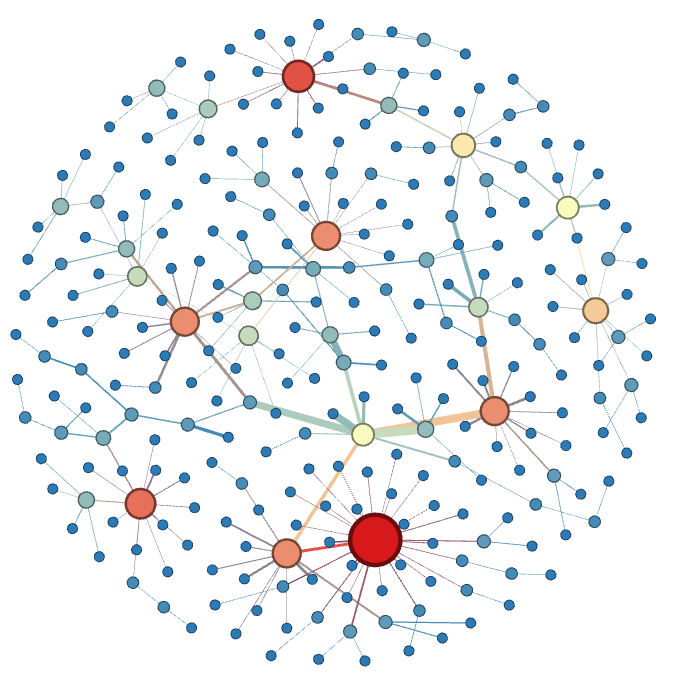
\includegraphics[width=0.25\textwidth]{../visualizacion/qn_fr_us}
            \label{qnfrus}
        }
    }
    \caption{Visualizaciones de las PFNETs del cienciograma United\_States-2002 realizadas con el método de distribución F-R}
    \label{frus}
\end{figure}

\begin{figure}[!h]
    \centering
    \mbox{
        \subfigure[PFNET($r = \infty$, $q = 2$)]{
            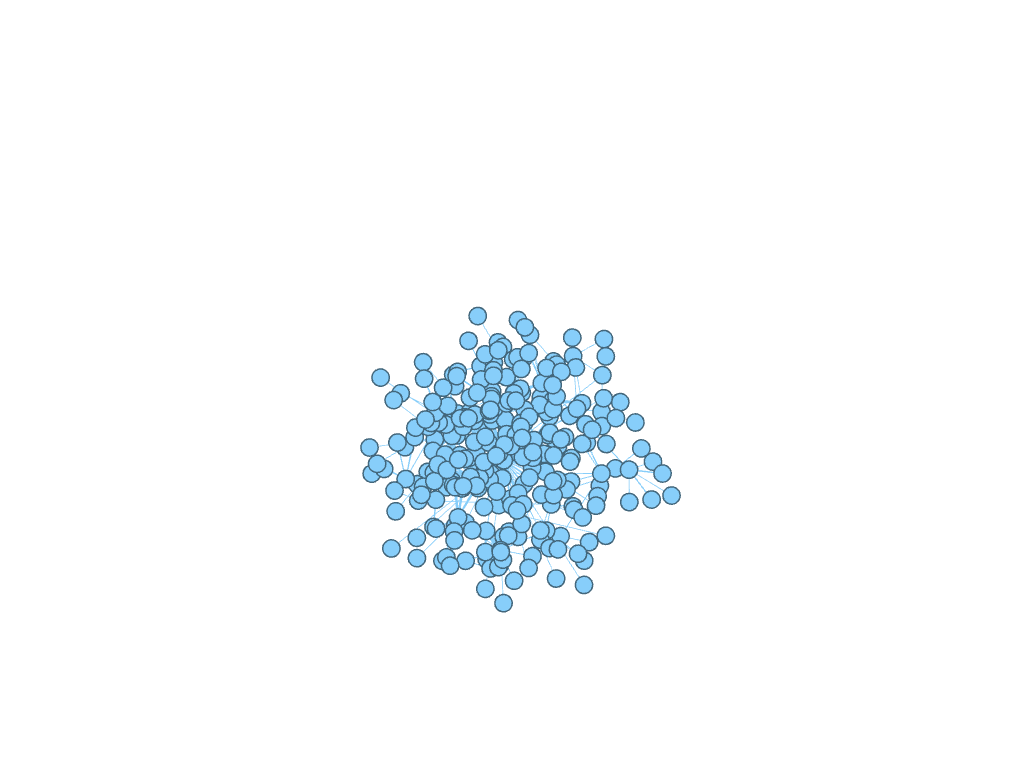
\includegraphics[width=0.25\textwidth]{../visualizacion/q2_kk_us}
            \label{q2kkus}
        }
        \subfigure[PFNET($r = \infty$, $q = 3$)]{
            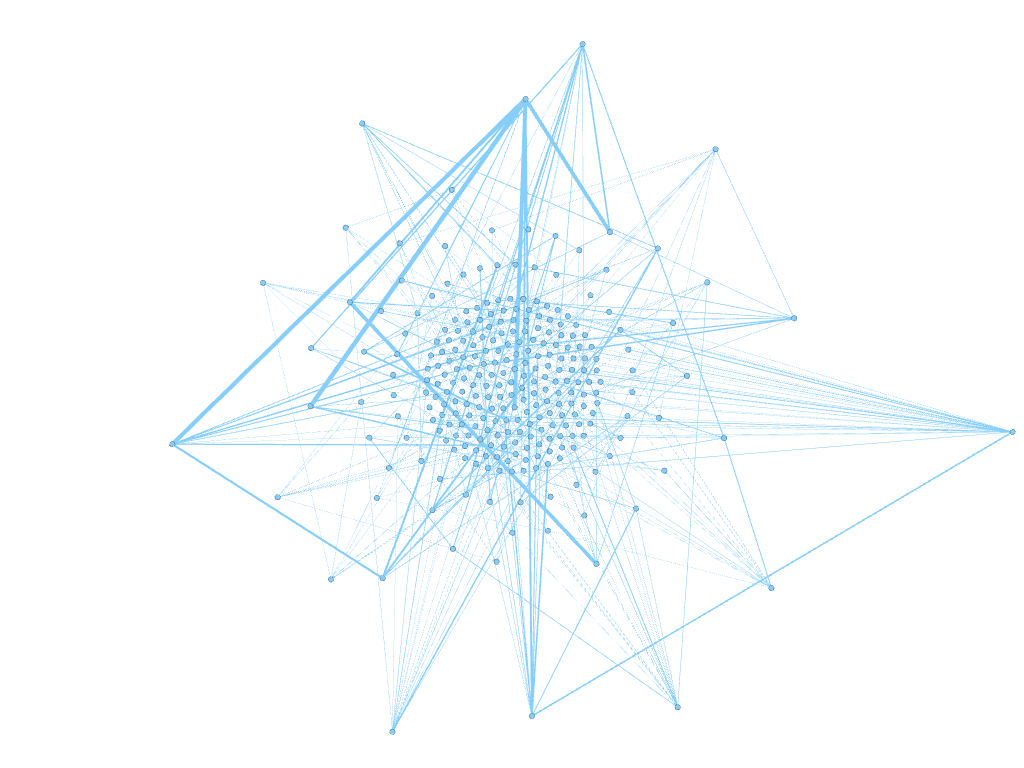
\includegraphics[width=0.25\textwidth]{../visualizacion/q3_kk_us}
            \label{q3kkus}
        }
    }
    \mbox{
        \subfigure[PFNET($r = \infty$, $q = 4$)]{
            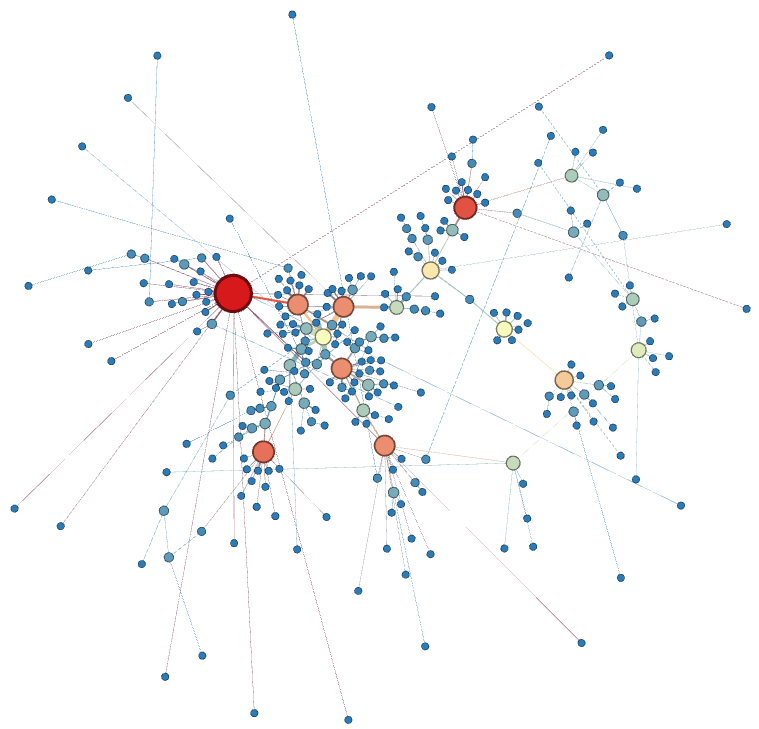
\includegraphics[width=0.25\textwidth]{../visualizacion/q4_kk_us}
            \label{q4kkus}
        }
        \subfigure[PFNET($r = \infty$, $q = n-1$)]{
            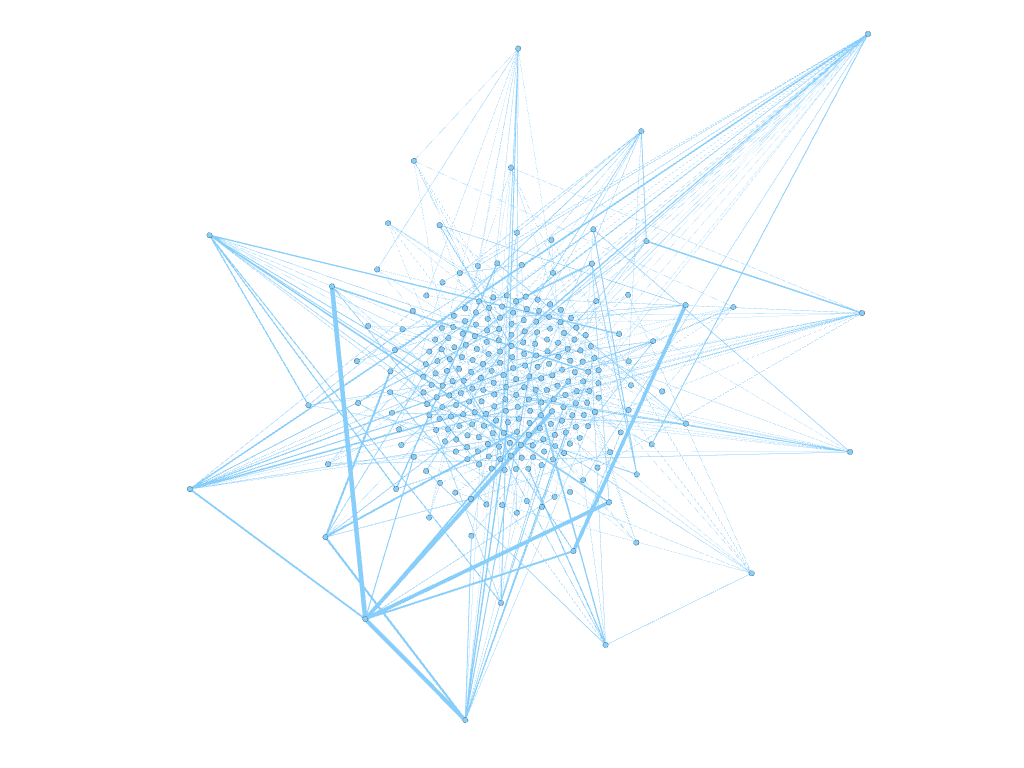
\includegraphics[width=0.25\textwidth]{../visualizacion/qn_kk_us}
            \label{qnkkus}
        }
    }
    \caption{Visualizaciones de las PFNETs del cienciograma United\_States-2002 realizadas con el método de distribución K-K}
    \label{kkus}
\end{figure}


\section{Análisis de la eficiencia de las distintas variantes de \textit{Pathfinder} en redes de gran tamaño.}
Para realizar las ejecuciones he hecho un script en \textit{Python} que genera las redes aleatorias usando el código C dado por el profesor y lo poda con las distintas variantes del algoritmo \textit{Pathfinder}. Como mínimo, la red generada tendrá $500$ enlaces y, como máximo $5000$. Además, la probabilidad de que exista un enlace entre dos nodos es de $0.5$.

\begin{table}[!h]
\begin{tabular}{rrrlllll}
\hline
    $N$ &    Media $L$ &   Media $D$ & Original             & Binary               & Fast                 & MST (Teorico)          & MST (Práctico)         \\
\hline
$500$ &   $1252$ & $0.0100$  & $82.9369$  & $6.3309$  & $0.4045$ & $0.0374$ & $0.0065$ \\
$1000$ & $4999$ & $0.0100$   &       $1304.4014$ & $89.3710$  & $2.9496$ & $0.0201$  & $0.0203$ \\
$2000$ &  $20041$ & $0.0100$  &       $> 1800$ & $1234.4935$ & $23.6252$ & $0.1561$  & $0.0792$  \\
$5000$ & $124525$ & $0.0099$ & $> 1800$ & $> 1800$ & $361.3296$   & $0.4194$   & $0.4552$   \\
$10000$ & $498666$ & $0.0099$ & $> 1800$ & $> 1800$ & $> 1800$ & $1.7304$   & $1.5963$    \\
\hline
\end{tabular}


\caption{Tiempos de poda de cada algoritmo}
\label{tiempopoda}
\end{table}


\end{document}

